\section{Product Development}\label{sec:product_development}
\subsection{Planing phase}
Before building the program, we brainstormed and created a Minimal Viable Product (MVP).
This MVP (which can be seen illustrate beneath) is a generally high-level schematic outlining what our program is supposed to do.

\begin{figure}[H]
  \centering
  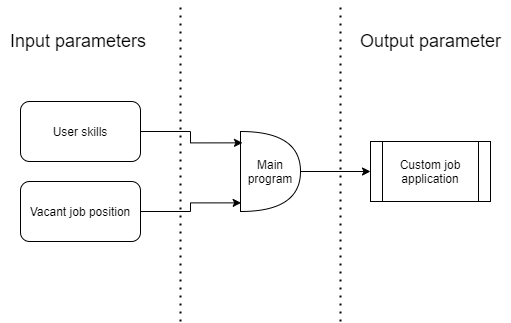
\includegraphics[scale = 0.6]{figures/engMVP}
  \caption{MVP}
\end{figure}
Here we discussed what were the most essential parts, and concluded that the following things
were needed: The user's skills/abilities and the information from the vacant job position. These things
should be transformed into a custom application. 

After further consideration, we had encountered a problem: That generating a custom CV from nothing but
skills/abilities would create a very childlike, maybe even unreadable, application. This could be solved with a lot
of data, and therefore a lot of time calibrating the process of automatically creating sentences. This may also result
in a lower quality application if this calibration doesn't happen. 
A CV, that might and might not even get through the "ATS/keyword scanner" outlined in the analysis. 

We, therefore, sought to instead create a filter, where the high-quality sentences would be somewhat guaranteed and maintained.
This filter is only supposed to filter out all the unnecessary parts of a longer quality CV, into an application that
is ready to be sent. In other words, we decided to instead concentrate on creating a tool that aids
in sending out applications, instead of a CV generation program.

We then changed the MVP schematic to the following:
\begin{figure}[H]
  \centering
  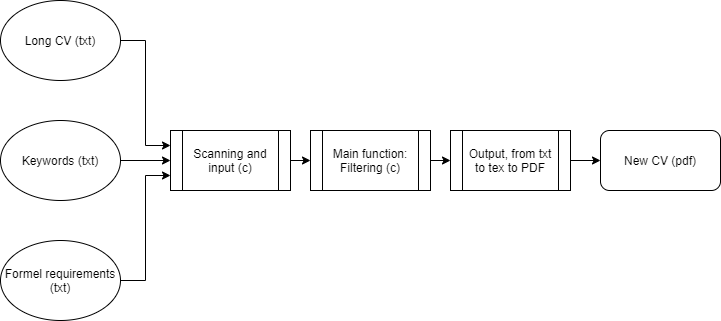
\includegraphics[scale = 0.6]{figures/Program_process_diagram.png}
  \caption{Revised MVP}
\end{figure}
This program is supposed to take in the keywords/job application, some formal requirements for
the structure of the new CV, and the originally long CV.
 
The long CV should contain as many pages as possible, of all abilities and skills one has.
It should also include prior work experience, and anything else relevant on a CV. 

In this way, the program chooses the most important sentences, work experience, and skills to be included,
and from the structural requirements creates a new CV.

From here we decided to organize our MVP into a UML diagram, to make it more apparent
what the essential functions were supposed to do, and which functions that were essential:
\begin{figure}[H]
  \raggedright
  \hspace*{-1in}
  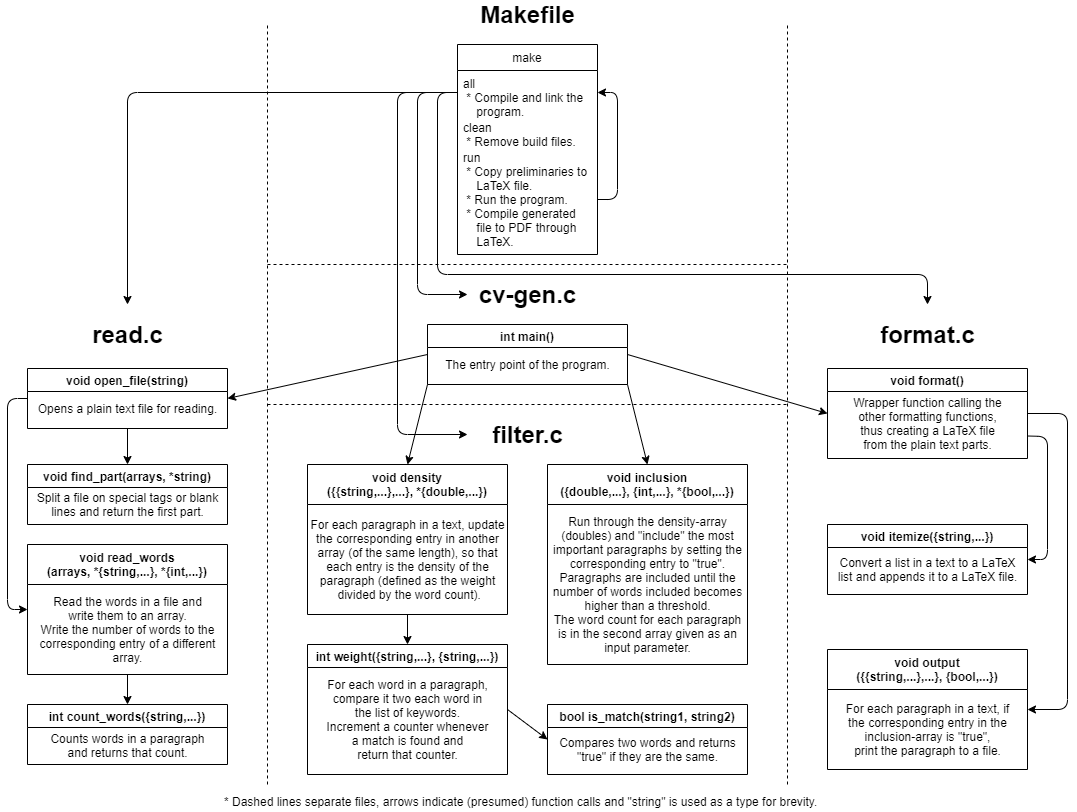
\includegraphics[scale = 0.50,left]{figures/UML}
  \caption{UML}
  \label{fig:UML}
\end{figure}
\newpage

\subsection{Read.c}
\subsection{Filter.c}
The filter file is the next step in the process to creating a new CV, after read.c has been executed.
The filter.c file has the following structure and interaction with the main.c file:
\begin{figure}[H]
  \centering
  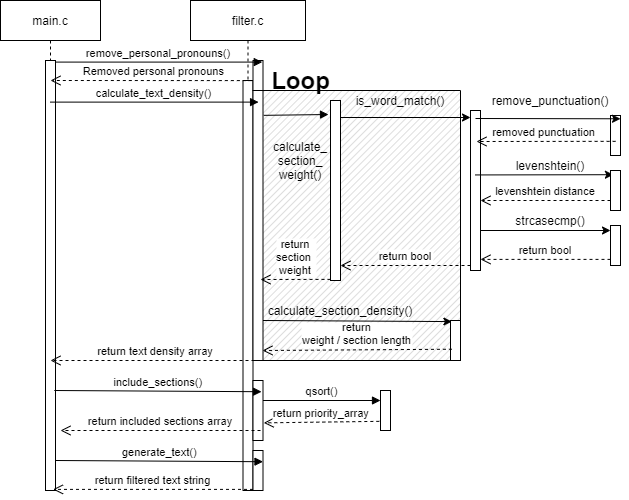
\includegraphics[scale = 0.6]{figures/filter_flow.png}
  \caption{Filter Sequence Diagram}
\end{figure}
The end result from the filter file will then later on be used in the format.c file.

\subsubsection{Removing Personal Pronouns}
After receiving the "free text" part, from the read.c file, we need to remove any personal pronouns.
We do this since personal pronouns are quite unnecessary since they don't add any substance to the sentences.
This is important to do since recruiters, as we talked about in the background section, spend a fraction of a minute
to look through the application. 
Having more unnecessary words will just distract the recruiters from understanding why they should hire you.
As talked about in the background section, not using personal pronouns increases your
chances of getting an interview by 55 percent.
\\
To remove all personal pronouns before filtering the rest of the text, we made the following function:
%\incfigure{figures/personal_pronoun}{fig: pp function}{Remove personal pronouns function}
\begin{figure}[H]
  \centering
  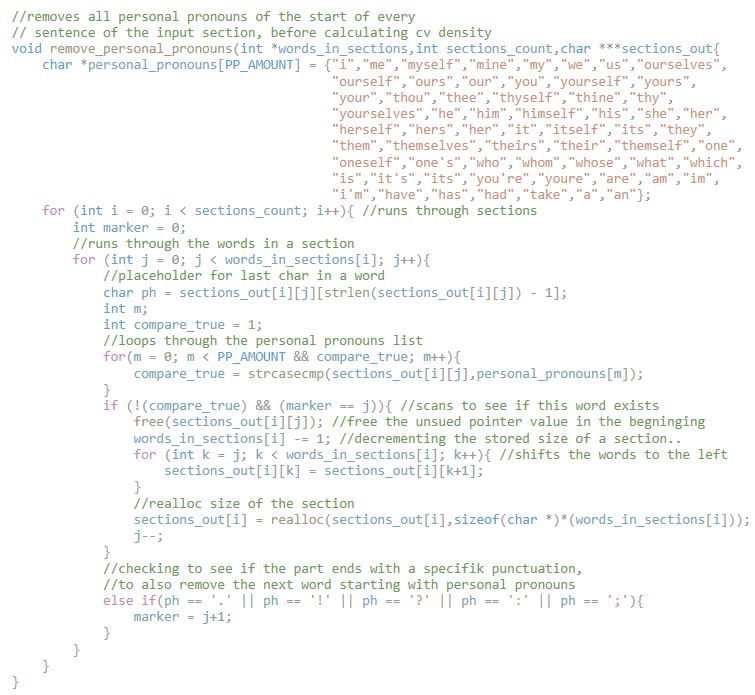
\includegraphics[scale = 1]{figures/personal_pronoun_v2.png}
  \caption{Remove Personal Pronouns Function}\label{fig:personal_pronoun_v2}
\end{figure}

It's a pretty simple function. To start it reads a certain section. Then it removes all personal pronouns at the start of each sentence in that section.
It loops through it until there is no longer any personal pronouns left.
\\
To identity which words are personal pronouns, we have hardcoded a list of personal pronouns\cite{english_personal_pronouns} (including some words that are also unnecessary), that will be 'case insensitive compared'.
Each time a word is identified as a personal pronoun, a loop swaps all the words 1 to the left in the array, where the last word in that array will then be freed.
\\
There are also some hardcoded punctuation symbols, to indicate what is defined as the "start of a sentence". 
\\
this results in the following:
\begin{figure}[H]
  \centering
  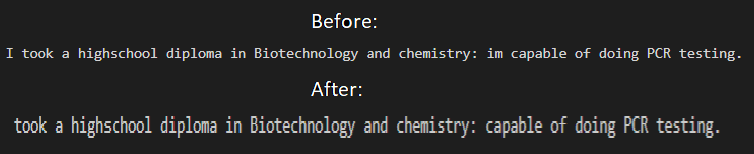
\includegraphics[scale = 0.6]{figures/personal_pronoun_ex.png}
  \caption{Removing Personal Pronouns Example}
\end{figure}
%\incfigure{figures/personal_pronoun_ex}{fig: pp example}{Removing Personal Pronouns example}

As we can see, the filtered result is much cleaner and easier to read, without losing any information.
There is the only problem left with it. Since the words are just shifted 1 to the left in the array, the sentence no longer begins
with a capitalized letter. This will later be fixed in a function in format.c, where such things will be formatted.

\subsubsection{Word Matching}
Word matching is one of the most interesting and most fundamental functions. 
It is the function that allows for keyword matching to existing, so that the application
may get through the ATS/keyword scan. How it works is it checks if input word 1, matches with the input of word 2.
Where input 1 is the unfiltered original application text and input 2 is the keywords for the job posting.
If it is a match, then one might have an idea, that this section where the matched keyword is included may be important.
It does this using the function strcmp(n,r), which returns 0 if the string (or in our case, word) is identical.
\\
One quickly stumbles upon the following problems trying to match keywords.
\begin{itemize}
  \item 1. Since letters are ASCII defined, when comparing "Bathtime" with "bathtime", it won't return it as a match, even though it is.
  \item 2. What if the word is the last in a sentence? Comparing "Bathtime." with "Bathtime" should return a match, but it won't.
  \item 3. What if one has made simple spelling mistakes, such as spelling "Twilight" with 1 'l' instead of the required 2 'l's.
\end{itemize}

To overcome the first problem, one could easily make a loop, loop through each letter, and check for both the capitalized and the small letters,
and return a match. This is especially easy since the small letters always have a 32 higher ASCII value from their capitalized counterpart.
But after reading through the string library we found a function that does just the same comparison while ignoring capitalized letters: strcasecmp(n,r).
\\
The second problem has quite a simple solution as well. Using the ASCII value of different kinds of punctuation symbols, we can easily remove these symbols by inserting a null terminator. 
instead, thus making the string shorter. This is done, on a temporarily saved word, such that this temporarily saved word can be used in the string compare function. This is done since we don't want to change the punctuation of the final output.
\\
The third problem is the trickiest one of the bunch. To solve this we decided on using an algorithm to find the Levenshtein distance. 
We found a translation of this algorithm in C and imported it\cite{levenshtein}.
The way this algorithm works is by finding the distance between words. The larger the distance, the greater the difference between the words.
The algorithm determines distance as the number of operations needed to change string A to string B. The algorithm uses 3 different types of operations:
\begin{itemize}
  \item 1. Insertion
  \item 2. Deletion
  \item 3. Substitution
\end{itemize}

to give an example of how these 3 operations can be applied:
\begin{itemize}
  \item Turn "Cat" into "Fat"  (Substitution, 'C' with 'F')
  \item Turn "Fart" into "Far"  (Deletion, removing the 'T')
  \item Turn "Sittin" into "Sitting"  (Insertion, adding a 'G')
\end{itemize}

as an example, the levenshtein distance between rain -> shine is 3, shine -> train is 4:
\begin{figure}[H]
  \centering
  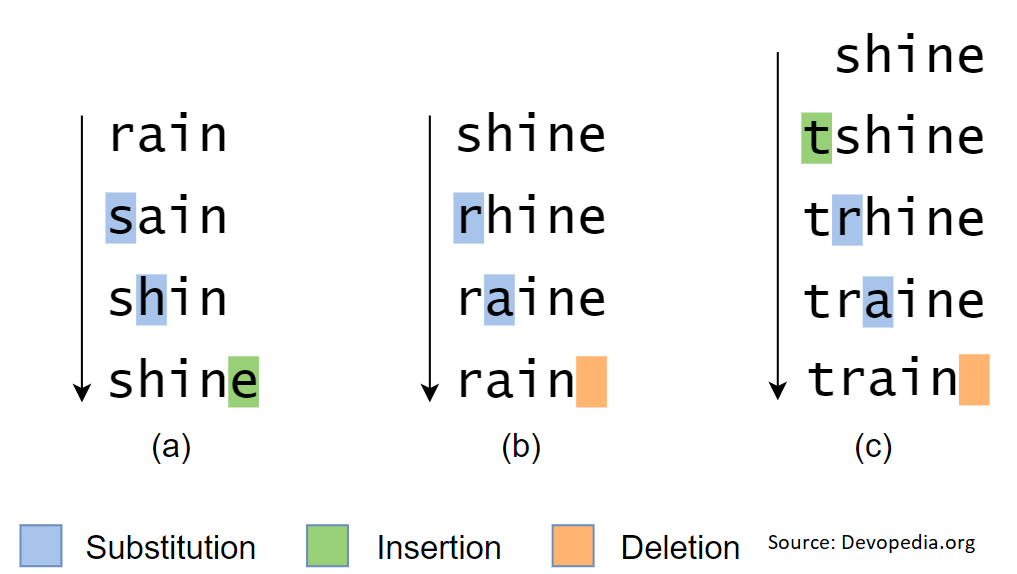
\includegraphics[scale = 0.6]{figures/levenshtein_example.png}
  \caption{example of levenshtein distance, \cite{levenshtein_distance}}
\end{figure}

The levenshtein distance can be defined using the following naive recursive definition where |a| and |b| is the distance of a and b respectively:
\begin{figure}[H]
  \centering
  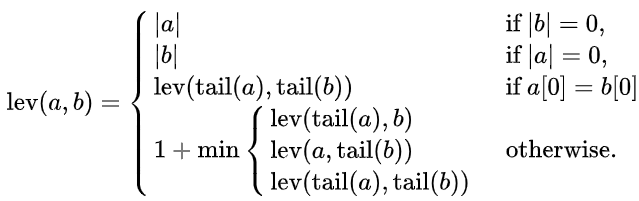
\includegraphics[scale = 0.7]{figures/levenshtein_recursive.png}
  \caption{Naive Recursion, \cite{levenshtein_recursive_definition}}
\end{figure}
The "tail" part is the entire word minus the first letter.
The base steps go as follows: It returns the length of an as the distance, if the length of word b is zero, and vice versa.
if the first letter of a and b equal each other, then it recursively runs the algorithm with the tail part of a and b.
Otherwise, it finds the minimum value (assuming the operations are weighted differently) of either operation 1 (Deletion), 2 (Insertion), or 3 (Substitution) and adds 1 to the result. \\

Using the Levenshtein distance quickly raises a problem though since the distance between cat and hat is smaller than the distance
between artificial and artificially. 
It's obvious that this isn't a spelling mistake, but 2 distinct words. Therefore we ran
some tests, to see how long words need to be before something like this doesn't happen too often. 
The problem quickly becomes, that the longer the requirement the better the accuracy. 
But also the fewer words we can use the algorithm on, making the algorithm redundant.
We came to the conclusion based on our tests, that having words with greater than 4 letters, would be
the best compromise between length and accuracy. \\

Now the problem is, what distance is accepted as 2 words being the same?
Here the problem also becomes, that grammatical endings are still the same words, just conjugated.
Based on a list of grammatical endings, the longest English ending adds a suffix of 3 letters\cite{grammar_endings}. Thus,
the max Levenshtein distance should be under 4 letters.
Retesting using these values, we find that in nearly all arbitrary cases, the Levenshtein algorithm matches the right words.
One problem may arise from the fact, that words can have different meanings in different contexts. Unfortunately taking account for semantics is out of the scope of this program. \\

After using the algorithm to find the Levenshtein distance, one could argue that the removed punctuation function is redundant. But this is not the case. On the contrary, removing any
unnecessary parts of a string before finding the Levenshtein distance, makes the algorithm more precise. This is the case since we can make sure the allowed distance
is smaller than what it had to be if we hadn't removed punctuation. \\

The overall structure of this functions ends up looking like the following: %is_word_match "SKAL VÆRE HER"
\newpage
The overall structure can be described as this:
\begin{figure}[H]
  \centering
  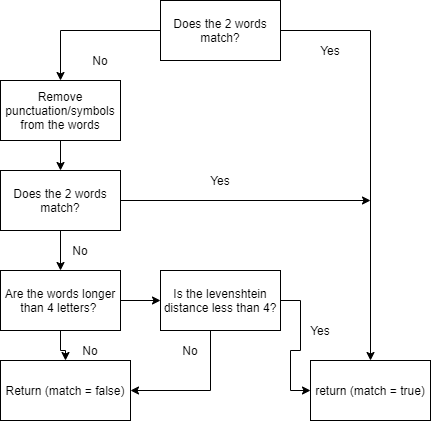
\includegraphics[scale = 0.55]{figures/is_match}
  \caption{Flow diagram of word matching}\label{fig:is_match}
\end{figure}

The structure is constructed as a chain of if statements, to avoid unnecessarily
calculations, so that the run time is optimized as much as possible.\\
\subsubsection{Section Density}
\begin{figure}[H]
  \centering
  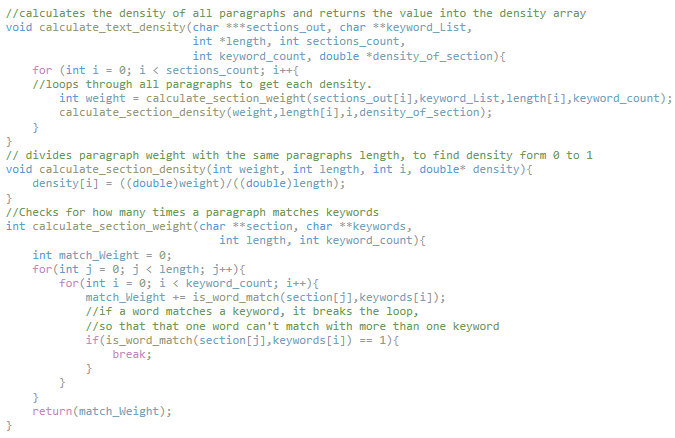
\includegraphics[scale = 1]{figures/section_density_v2}
  \caption{Density and weight function}\label{fig:section_density_v2}
\end{figure}
Section density is based on the same concepts as in physics: Weight(mass)/Volume = Density.
In this case, weight is how many times in a section different words match with a keyword, and volume is how many words there
are in a section. The boundaries for the density function is as follows: Density goes from zero to one. 
Where zero is that there are no matches in a section, and one, is that every single word matches. Though a problem quickly arises
from doing it this way: A word may match with multiple keywords.\\
\begin{itemize}
  \item Section: "physic expert", keywords: "Physics, physical".
\end{itemize}
Since the Levenshtein distance is only 3 between physic and physical, and 1 between physic and physics,
the word physic will match with them both, thus potentially creating a section with a density higher than the allowed 1.
To fix this issue, there was made a break condition for the weight loop, if a word from the section matched with a keyword.
The break function makes it such that no word could match with more than 1 keyword.
\\
Once the section's density has been calculated, the calculated density will be saved chronologically in a calloc'ed array of double values. 
This will be used to access which sections are the most "important", from the definition that the more keyword matches, the greater the importance.
\\
Printing the result from this, we can see:
\begin{figure}[H]
  \centering
  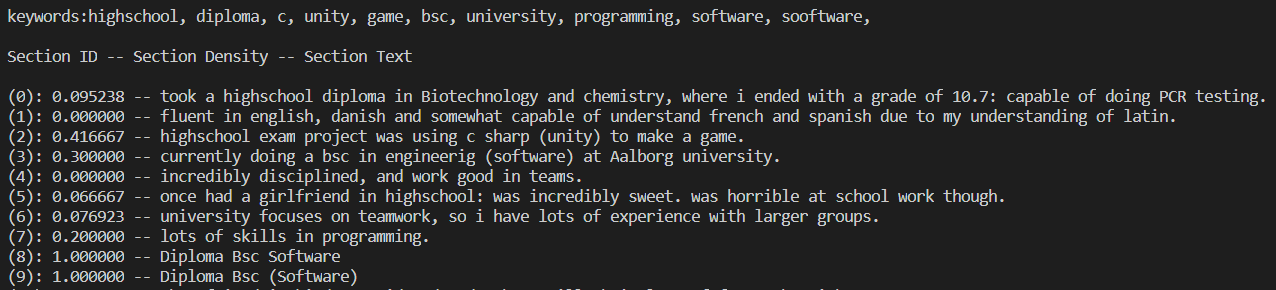
\includegraphics[scale = 0.6]{figures/density_example.png}
  \caption{Density Array Printed}
\end{figure}
%\incfigure{figures/density_example}{fig: density example}{Density array printet}
Thus it can easily be seen, which sections may be best suited for the job opening. 
In this case, an example of a job opening specializing in software.

To demonstrate that the functions work, it can be seen that both line 8 and 9 get printed with a result of exactly 1.
Even though one of the words match with 2, and the other, though misspelled, also matches with 2.

\subsubsection{Included Sections and Generation}
%\incfigure{figures/includefunction}{fig: inclusionfunction}{Inclusion Function}
\begin{figure}[H]
  \centering
  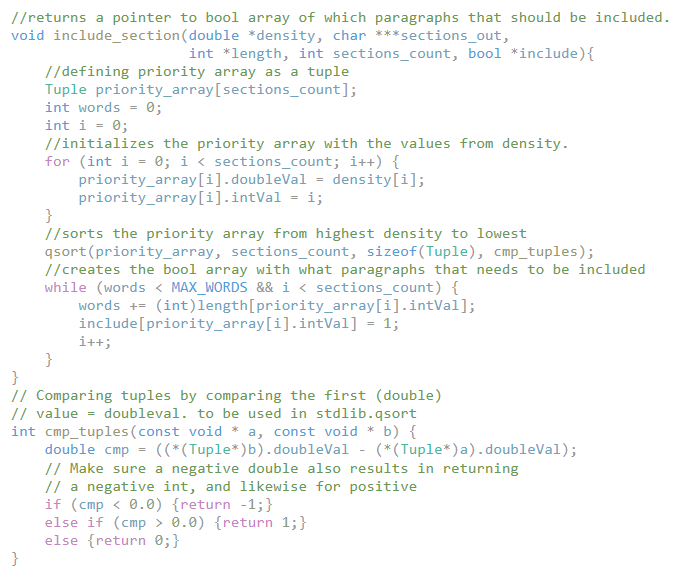
\includegraphics[scale = 1]{figures/includefunction_v2.png}
  \caption{Inclusion Function}\label{fig:includefunction_v2}
\end{figure}
The process of finding the included sections can be described in three steps:
\begin{itemize}
  \item 1. Create a tuple struct holding the density value, and the section ID.
  \item 2. Q-Sort the struct after density value.
  \item 3. save what section ID's should be included in the final output, based on the density, in a bool array.
\end{itemize}
First, a struct is created. This is to ensure, that after sorting after the highest density, the original order is still maintained.
This is important since it can make it unreadable if all the sections are confusing. 
After that, a Q-sort algorithm is used from the standard library. This algorithm makes sure, that the highest density comes first, by sorting by densities.
Q-sort is based on quicksort, which is a type of divide and conquers algorithm. Which as the name suggests, divides the list (array) into atomic parts, and conquers the parts, such that the new list is sorted.
\begin{figure}[H]
  \centering
  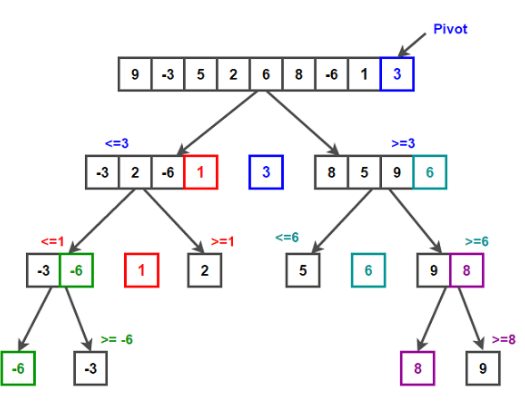
\includegraphics[scale = 0.7]{figures/qsort.png}
  \caption{Quick Sort \cite{quicksort}}
\end{figure}
The way it works is that it chooses a pivot point, traditionally randomly, the leftmost or the rightmost element.
In more modern versions of quicksort, the pivot point is chosen as the median. The rest of the list is then divided up into 2 lists.
The elements of the 2 lists are chosen by whether there are smaller or larger than the pivot point.
A new pivot point is selected, and this process continues until each list only contains one element. 
Then the elements can be recombined in the new order, and thus the list (array) is sorted.
\\
Next, a bool array is created and calloc'ed. The values for the bool array are determined following this flowchart:
%\incfigure{figures/include_flow}{fig: inclusion flowchart}{Flow diagram of the bool array}
\begin{figure}[H]
  \centering
  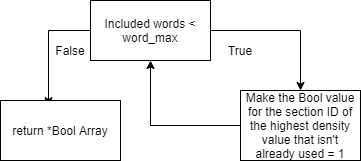
\includegraphics[scale = 0.6]{figures/include_flow.png}
  \caption{Flow Diagram of the Bool Array}
\end{figure} 
%\newline
To determine what sections should be included, a while loop is run, until a certain amount of words are included.
The amount of allowed words in the output is restricted to around 650, as that is the range, which grants the most amount of interviews.
That is, according to the research as described in the background section.
\\ \\
Here is an example, of it, working: 
%\incfigure{figures/bool_example}{fig: bool diagram}{Example of the bool array} 
\begin{figure}[H]
  \centering
  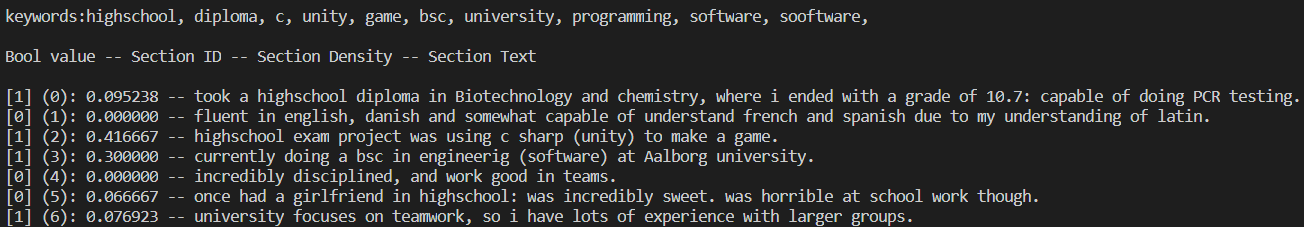
\includegraphics[scale = 0.6]{figures/bool_example.png}
  \caption{Example of the Bool Array}
\end{figure}
The generation of the cv is quite simple in theory. All it does is include all sections that the bool array determines should be included and saves it into a long string.
Starting from the lowest section ID to the highest ID. \\
The process of getting here is a little more complex since it requires a lot of dynamic arrays, and inserting a lot of Null terminators, such that it doesn't print null pointers (I.e "(NULL)" ).

%This part isn't that interesting, but if you're interested, you can see it here:
%\incfigure{figures/generate}{fig: generate function}{Text Generation Function}
%\begin{figure}[H]
%  \centering
%  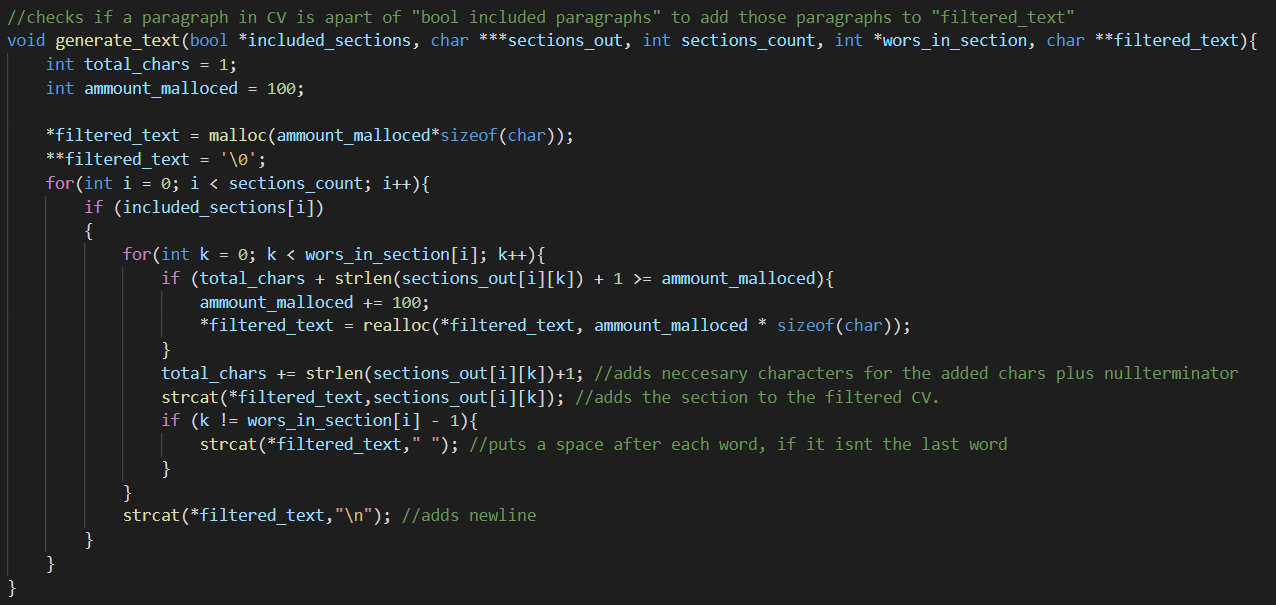
\includegraphics[scale = 0.6]{figures/generate.png}
%  \caption{Text Generation Function}\label{fig:ie}
%\end{figure}

\subsection{Format.c}
After the CV has been filtered, our next plan is to print out the text to a LaTeX format, and afterward compile it to a pdf file. 
This program will check the format and edited it accordingly to how a CV should be visualized. 
There are several step before entering the main function for format.c,
and it's done accordingly to this diagram.
\begin{figure}[H]
  \centering
  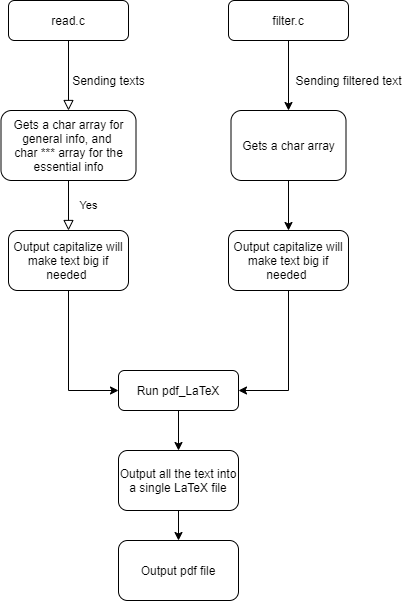
\includegraphics[scale = 0.6]{figures/Fra_read.c_og_filter.c_format.c}
  \caption{Flow diagram for coming to format.c}
\end{figure}

\subsubsection{Output Capitalized}
The first function will capitalize any letter that has a dot, question mark, or an exclamation mark.
The function has one variable, a char array to check after characters if these need to be capitalized,
it can therefore be useful for all the contents in the CV - the general information, education, work experience, or free text.
There are two integer markers to indicate the index of an array, 
and right now, it's outside of the index, so the markers will not have access to the first index in the array,
since it doesn't need to be for finding text, as long as the file is being read.
To see the length of a string, a function called strlen will know how long is a string. \\

A string can be a sentence, and every time the first letter will always be capitalized,
and it can be done so with toupper.
This is a function that is included in the c-type header.
After a sentence is finished with a dot, question mark, or an exclamation mark, 
the letter is always capitalized after those markings.
For doing line breaks in LaTeX it only needs two backslashes, a par or a newline command. 
To these above properly for a full text, a for loop needed to check the length of the char array,
it will do so by -1 with it because it has to end at an exclamation point before the null terminator.\\

The integer 'i' should always go up by 1 if it's still lower than the length, 
and that means until the text is finally done it will continue to capitalize letters. The capitalized letter will only capitalize on two scenarios, 
the letter will be either after space, and if there is a line break.
There is also a chance if the text turns up to have a dot, question mark, or an exclamation mark like described before.
This will let the marker index 1 and 2 have their value changed by +1 since the program will afterward look for space.\\

\subsubsection{LaTeX general Contents}
The most crucial part is how to output the entire text from for example an ordinary txt file to LaTeX format.
output general contents have a char array that will take the whole section from general contents and added it in the CV,
also, there are a file handling variable as well to output the text to a specific file. 

The function output capitalized is included in this function, if the text needs to capitalize.
Finally, the general text will begin at the center with a LaTeX command, follow up by a minipage command, 
and at last make the text width smaller, so the text will be moved more at the left side, and the title is auto-generated. \\

General contents from read.c will not be sorted after keywords or anything similar since the name, address, e-mail, etc. is important to let the recruiters know and therefore it should not be filtered from filter.c.
The output of the text will be a string from the char array 
and end it with a minipage and hfill - the unused lines will be used by this command in LaTeX.
After hfill has been executed, the output of a picture begins a minipage 
and then prints out a picture with includegraphics, and it is been programmed to be right beside the general info. 

\subsubsection{handling essential contents and free text}
Essential contents have a char array with three-pointers to check the sentences,
the words, and last with the letters to get an opportunity for adding educations and work experiences.
These will therefore have an n-amount of itemizes and n number of items in an itemize, 
and item and itemize is a form for putting bullet points.
The program will start printing out the self-selected subtitle and n number of itemizes.
Texts under a hashtag are being loaded from read.c and it will afterward be sent to a LaTeX CV.\\
 
To check the amount of itemizes for the essential contents it will use a for loop to check each value,
and after the 'i' is bigger than the amount of itemizes the loop will stop - the amount of itemizes is coming from read.c.
After having checked hashtags and the text as well, and hashtags are for indicating the sections,
this way the array essential contents variable will therefore have a 2-dimension array.
The same goes for the number of items to output because there can be n amount of jobs to writes, 
therefore, the program is using a for loop to run down after how many jobs have been transferred from read.c.
The arrays has also 2 dimensions, first for checking the amount of itemizes [i] and for the number of items [j] in the indexes.
when there is no need to make more items and itemizes the for loops will stop and end the functions. \\

As for the free text and this is where the most common for background information if this relevant for the specific job.
This only function that is being filtered by filter.c. It is fairly simple, 
the text that is being received is a char array and will therefore be treated as a string 
just like before for the general information. All information is going to the CV file at the end of the function.
It will have a static title so it is not going to be edited.

\subsubsection{Run the whole LaTeX document}
When all of the functions above are created this function will then call all other function and run it add all the text into a file,
and build the document into LaTeX and later on a pdf file.
First of the function will create or overwrite a file if possible. There can be various kinds of reasons why a file can't be created.
If the file can't be opened then it will be the end of the program with "EXIT FAILURE", 
and it will go out with a message "Cannot open file".
As long as the file is created or overwritten the rest of the program will run.\\

There is included a preamble and this will enhance the LaTeX format readability for the user and recruiter when reading it. 
Most of the time a picture of oneself is required for most of the jobs, therefore it is possible to manually insert a photo to the CV. 

\subsection{Main.c}
As the program is heading to the final phase, all other c programs will be added to a large file, 
this is going to become the main.c, and it will have read.c, filter.c and format.c included for printing out the CV pdf file. \\

The program will start by running the start read. In this particular function, it will load out the whole file, 
similarly speaking it will split a complete text up to four separate if possible. A section is the biggest part of a text, 
therefore it will start with checking how many sections, then the sentences, words, and letters at last.
This function will also do the job to load out all the necessary bullet points, keywords, and word count. \\

In the filter.c it has four functions included in the main file.
At first, it has to check which sentence is best. A sentence length can be as long as it is, 
there in conclusion we have used calloc as a way to make a dynamic memory space for both "density of section" and "included section".
It can be tiring to have a lot of "i" in a CV, therefore remove personal pronouns is also included to remove those pronouns
, and will check a whole section for every time there is at least one pronoun. \\

calculate text density will calculate each string from the free text (background information) to see
if a keyword is matching any words in a sentence.
When this is done the include section function is checked with help of boolean values.
These values are consisting only of 1 and 0, 1 is true while 0 is false in the programming language.
Afterward, these selected texts will be generated by generating text, 
and that is the last part of the filter function before heading to format.c. \\

For creating a CV LaTeX file, it is going to run all the functions for general information, work experience information, 
education information, and the free text (other background information). After the function has printed out the CV pdf file,
it will come to a close with freeing all the variables of those were malloc, realloc, and calloc, 
so all of them don't continue to allocate more memory. All of those were will also apply to the "the ending" function.


Below the whole program is explained in a simple graphic method about what the main.c file contains 
in which order to execute the numerous aforementioned functions.
It follows a generally chronologically imperative flow:
\begin{figure}[H]
  \centering
  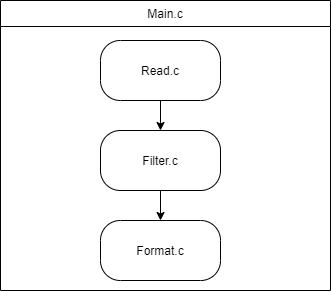
\includegraphics[scale = 0.6]{figures/main.png}
  \caption{Flow Diagram of main.c}
\end{figure}
\subsection{Makefile}
To compile the entire program, a makefile has been made. It links the header and .c files together, to create object files. Which are then compiled into one file named "generate cv".
This newly compiled file, when executed, can include the user picture, the user made keywords.txt and the user made long cv.txt, and from there create a pdf file.
This means, that the user mealy has to execute one file, for the program to work.

\subsection{TKOP-model}
A good way to describe the production could be the TKOP-model also known as technique, knowledge, organization, and product.
It gives an easy impression of what the project group had performed.
First is the technique, it is essential to create a product for our project to find a solution. 
one must use several techniques including C-programming, LaTeX, and GitHub techniques, researching on the web, etc.
Those techniques are a good way to establish a project solution. C-programming can help us to produce a CV using the techniques
of commands, functions, etc. LaTeX can give a monotonous structured format all the text is always the same. \\

These functions take one to have a fair amount of knowledge to make a LaTeX text properly.
First of all knowledge about a CV is important, and how to use the knowledge is also important.
Therefore it's best to start research about programming online that we don't know about, 
and afterward, the gained information will be used to implement our code and see if it's working. 
If not, then it's best to research more about the exact problem.
This is the same way the waterfall model is being used.
We don't exactly use it directly but it is a way to be finished with the code.
\begin{figure}[H]
  \centering
  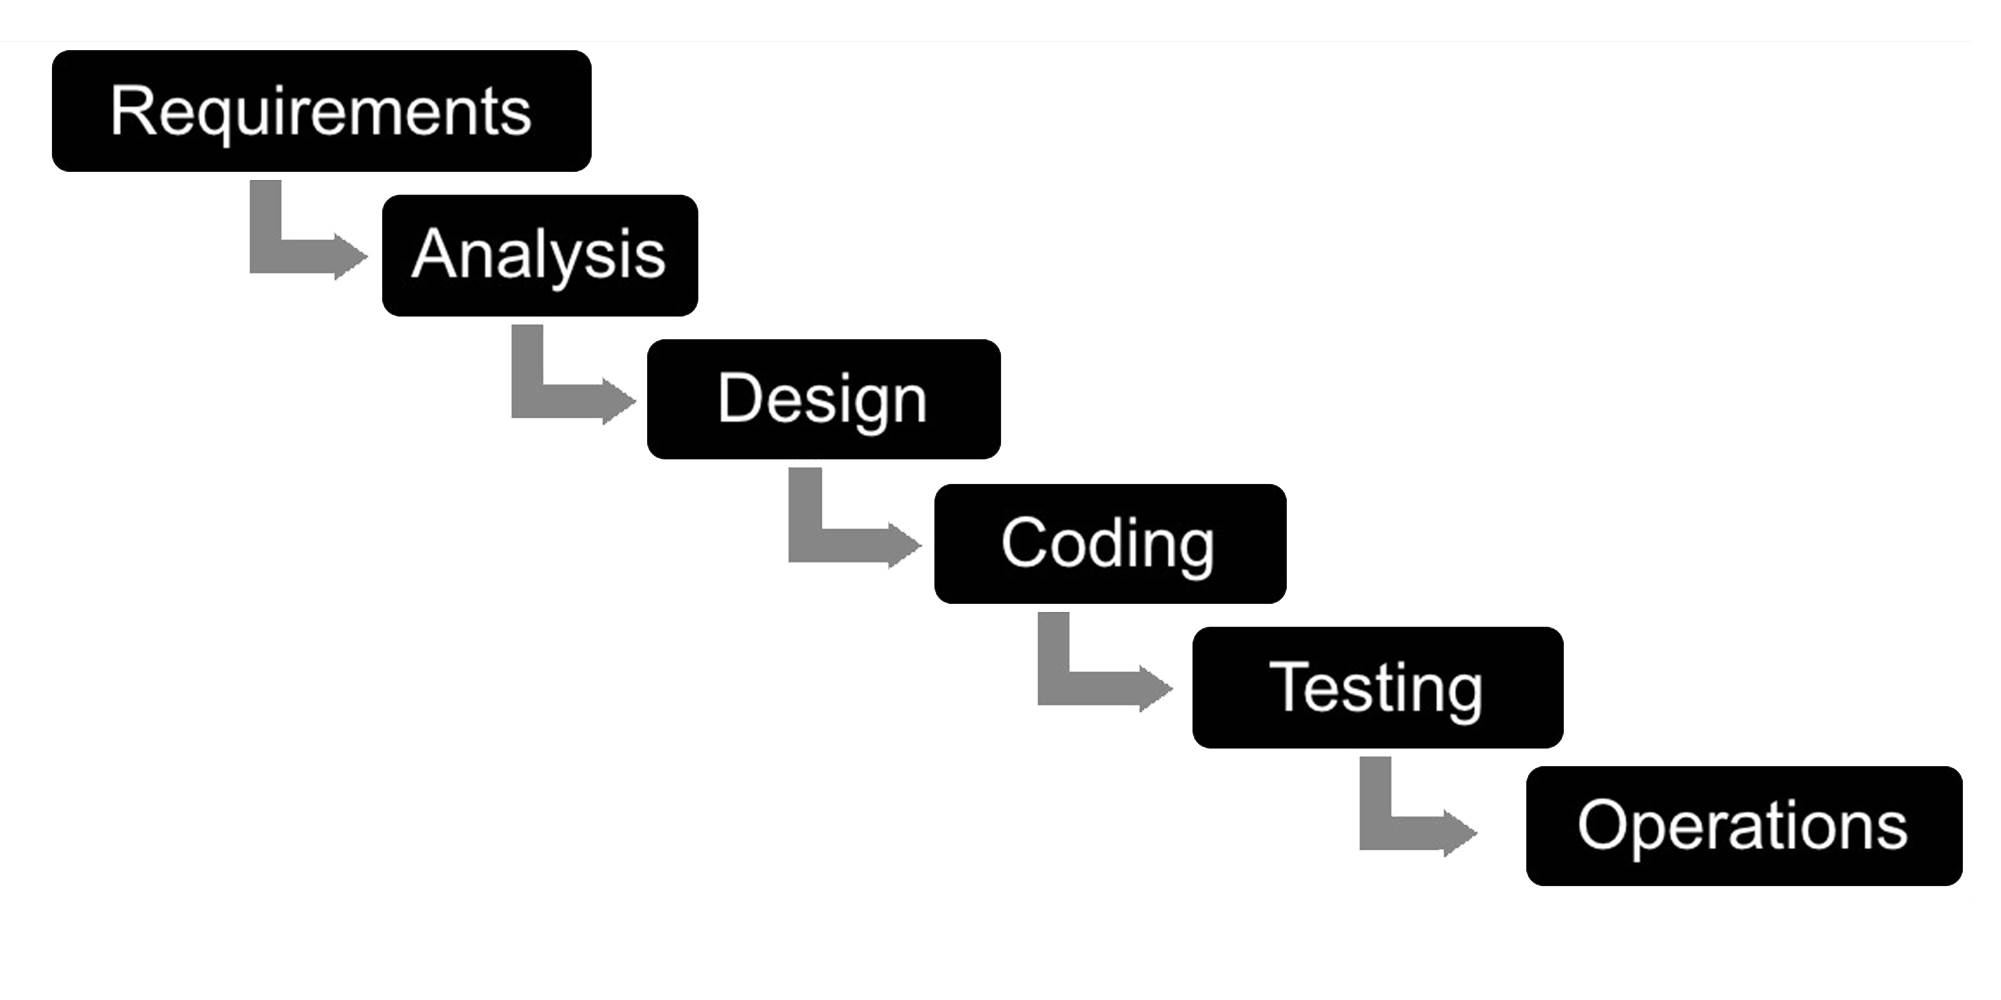
\includegraphics[scale = 0.2]{figures/vandfald}
  \caption{Waterfall model \cite{Waterfall_model}}
\end{figure}

It has the elements that have been implemented in our coding. First, we have the requirements for the program, 
so we can have a program that is working properly, 
next, we will design the structure of the program just like from the UML diagram in figure \vref{fig:UML}
 
so we know what should have in the program. Implementation comes next, so we could test the program later, 
and if we have other suggestions for improvement we can write them down for further development.\\

In the process of coding the product, we choose to use a vertical work distribution, as many of the product
components can be made parallel to each other. We divided it into several functions, 
so the group members can either do it alone or in pairs for each function to work with.
Each small group has to know future updates about the function development, so the program can be put together later on.
To get an overview of what we have done, there is a temporary division of labor for the schedule, 
so the group can see who is finished and what can be finished. \\

At last, our product is a program from C that will help to generate a CV. This way the CV can be made multiple times,
which means the use-value will be very high for the applicant will have a greater chance of getting a job interview,
rather than an ATS scanner will decline a CV, even though the text is very detailed with a lot of good points.
The C-program itself will not make the CV but it is an extension of a complex way to load from the other text editor
other than LaTeX, then compile it to LaTeX, so the tex file will make a pdf for the person.\\

If the whole process should be looked at different levels then there are five of them:

\begin{enumerate}
  \item Our program should be researched in four different aspects 
  \begin{enumerate}
    \item Knowledge to find the rights methods 
    \item Techniques to develop the product
    \item A strategy to give every single person a piece of the project, so all have an issue to work with.
    \item Knowledge about the product itself, and summarize the parts from all the issues to make a final product.
  \end{enumerate}
  \item Knowledge about the product of creating a CV.
  \item After gaining the knowledge,
        we can start coding for our software solution with help of programming techniques
  \item Our product has a long code with more function than the group itself, 
        Organize for each individual in the group is the key to get the project done faster.
  \item After making the product comes the testing where it can be done with help of experts CVs.
        This process will afterward lead to testing with the applicants if it is good enough for our criteria.
        All the coding parts will be added together in a readable way, and summarize all of it into a pdf file from a makefile.
\end{enumerate}